\documentclass[a4paper,10pt,twocolumn]{article}
\usepackage[utf8]{inputenc}
\usepackage{amsmath}
\usepackage{amsfonts}
\usepackage{amssymb}
\usepackage{graphicx}
\usepackage{braket}
\usepackage{sectsty}
\usepackage{biblatex}
\usepackage[font=small]{caption}

\addbibresource{quantum.bib}
\numberwithin{equation}{section}
\renewcommand\thesubsection{\alph{subsection}}
\newcommand{\bvp}[1]{\mathbf{#1}'}
\newcommand{\bv}[1]{\mathbf{#1}}

\sectionfont{\fontsize{10}{10}\selectfont}

%opening
\title{Mechanical coupling of microwave and optical photons}
\author{Vincent Baker, Drexel University Department of Physics}

\begin{document}

\twocolumn[
\begin{@twocolumnfalse}
 \maketitle
 \begin{abstract}
  Quantum electromagnetic phenomenon are of both theoretical and practical interest. 
  Quantum phenomenon are more readily observable at high energies where individual photons are well localized.
  New methods of coherent coupling between optical and microwave systems hold the promise of extending quantum techniques into the microwave regime. 
 \end{abstract}
\end{@twocolumnfalse}
]
\section{Introduction}
Coupling between optical and microwave modes creates a new set of experimental techniques to explore the principles of quantum dynamics.
The coherent transfer of quantum states may be exploited in applications including quantum-enhanced sensing and quantum computing.
Several similar mechanisms for optical/microwave coupling have been reported recently \cite{nanoCrystal, nanoMR}.\\
We will start by reviewing some of the proposed methods for microwave/optical coupling.
We then sketch the analytical exploration of the nanomechanical resonator from \cite{nanoMR} to demonstrate some important aspects of the approach. 
A general discussion of applications is followed by a discussion of aspects of quantum illumination applied to radar systems.

\section{Optical/Microwave Coupling Methods}
Several methods for coupling optical and microwave systems have been investigated. 
In \cite{nanoMR} the authors propose coupling microwave and optical cavity modes through a mechanical resonator.
The resonator itself is a drum-head capacitor that is coupled to the microwave cavity through a planar spiral inductor. 
The equivalent electrical circuit is resonant at microwave frequencies.
One surface of the mechanical resonator is coated with a mirrored finish and caps the end of an optical cavity.
The optically-induced mechanical motion changes the capacitance of the microwave resonator circuit, providing the desired coupling.
\begin{figure}[ht]
 \caption{Optical and microwave cavities entangled through a mechanical resonator. A, Proposed experimental setup. B, Equivalent circuit diagram of microwave resonator.}
 \centering
   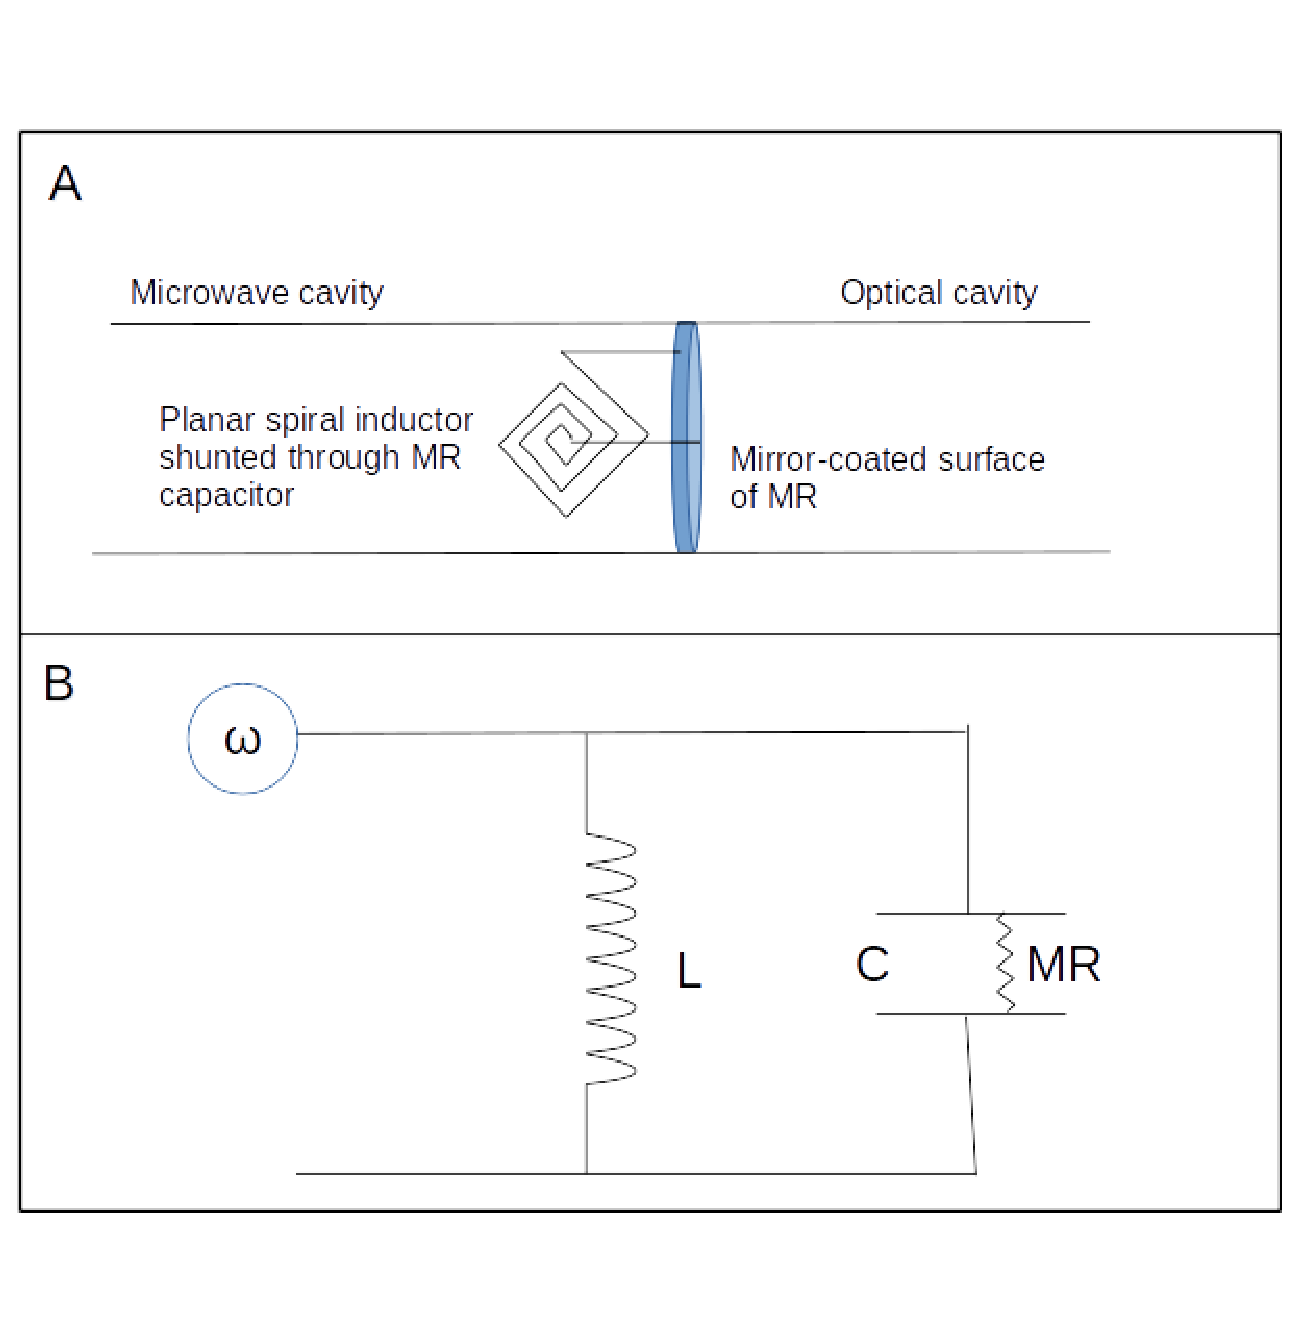
\includegraphics[width=0.5\textwidth]{f1}
\end{figure}
\\In \cite{nanoCrystal} the authors have characterized a coupled microwave/optical system using a piezoelectric optical nanocrystal.
\\
\section{Analysis of the Mechanical Resonator}
We present the analysis of the nanomechanical resonator system in \cite{nanoMR} to illustrate some of the relevant analytical methods.
The Hamiltonian of the combined system is expressed in terms of the creation and annihilation operators of the optical and microwave cavities.
The effects of thermal noise are incorporated through a set of quantum Langevin equations, which are then linearized about a stationary point. 
Finally the correlation matrix of the system is developed, from the which the logarithmic negativity can be calculated.
The log-negativity is a measure of the degree of entanglement between the elements of the system, and the results demonstrate the entanglement between the optical and microwave modes.
\\
We treat the nanomechanical resonator as a one-dimensional harmonic oscillator. 
We use the subscripts $w,m,c$ to denote parameters of the microwave cavity, mechanical resonator and optical cavity respectively.
The cavities are driven at frequencies detuned from resonance by $\Delta_{0w}$ and $\Delta{0c}$.
The Hamiltonian of the system shown in figure 1 is then:
\begin{align}
\begin{split}
 H = &\frac{p_x^2}{2m}+\frac{m\omega_m^2x^2}{2}\\
     &+\frac{\Phi^2}{2L}+\frac{Q^2}{2(C+C_0(x))}-e(t)Q\\
     &+\hbar\omega_c a^\dagger a-\hbar G_{0c}a^\dagger ax\\
     &+i\hbar E_c\left(a^\dagger e^{-i\omega_{0c}t}-ae^{i\omega_{0c}t} \right)
 \end{split}
\end{align}
Where $a^\dagger,a$ are the creation and annihilation operators of the optical cavity, $\Phi,Q$ are the flux through the inductor and the charge on the capacitor,
$e(t)=-i\sqrt{2\hbar\omega_wL}E_w\left(e^{i\omega_{0w}t}-e^{-i\omega_{0w}t} \right)$ is the driving function of the microwave cavity
and $G_{0c}\frac{\omega_c}{L}\sqrt{\hbar/m\omega_m} $ gives the optomechanical coupling rate with resonator mass m and optical cavity length L.
\\
The quadratic form of the microwave resonator circuit is amenable to expression in terms of microwave creation and annihilation operators $b,b^\dagger$.
We can then work in the interaction picture with respect to:
\begin{align}
 H_0 &= \hbar\omega_{0w}b^\dagger b +\hbar\omega_{0c}a^\dagger a
\end{align}
We can now express the time-dependent Hamiltonian in terms of the cavity detunings and neglect higher-order terms at $\pm2\omega_{0w},\pm2\pm\omega_{0c}$ since they will oscillate quickly and tend to average out.
The final Hamiltonian is:
\begin{align}
\begin{split}
 H = &\hbar\Delta_{0w}b^\dagger b+\hbar\Delta_{0c}a^\dagger a\\
     &+\frac{\hbar\omega_m}{2}(\hat{p}^2+\hat{q}^2)-\hbar G_{0w}\hat{q}b^\dagger b-\hbar G_{0c}\hat{q}a^\dagger a\\
     &+i\hbar E_w(b^\dagger -b)+i\hbar E_c(a^\dagger -a )
\end{split}
\end{align}

\section{Applications of coherent optical/microwave coupling}
Quanum computing.\\
Quantum illumination.
\section{Discussion of quantum radar}
Quantum-enhanced sensing is a relatively young field that seeks to enhance sensing by using quantum entanglement. 
We discuss the particular application of quantum illumination in the microwave regime applied to radar systems.
Radar systems determine the range, bearing and velocity of an object by emitting a microwave signal and measuring the signal reflections.
Radar waveforms are designed to allow the receiver to correlate the return signal from an object of interest in the presence of thermal noise, interfering signals and signal reflections from other objects.
Quantum illumination can improve this correlation and can theoretically provide better performance than any conventional microwave system. 
\\
Following \cite{qi} we look at the theorectical improvement over a classical system. 
We will then examine several challenges for quantum illumination, including pulsed waveforms and antenna arrays.
\printbibliography
\end{document}
